\documentclass[twocolumn]{article}
\usepackage{algorithmicx}
\usepackage{algpseudocode}
\usepackage{algorithm}
\usepackage{amsmath}
\usepackage{amssymb}
\usepackage{amsfonts}
\usepackage{stmaryrd}
\usepackage{hyperref}
\usepackage[pdftex]{graphicx}

\newcommand{\leaves}{\mathit{leaves}}
\newcommand{\branches}{\mathit{branches}}
\newcommand{\desc}{\mathit{desc}}
\newcommand{\bleft}{\mathit{left}}
\newcommand{\bright}{\mathit{right}}
\newcommand{\bbox}{\mathit{bbox}}
\newcommand{\broot}{\mathrm{root}}

\title{Building Better BVHs by Using Ray Distributions}
\author{Nicolas Feltman}

\begin{document}
\maketitle
\section{Introduction}
The naive way to trace a ray is to test it against each primitive in the scene and report the intersection closest to the source of the ray.  This is of course $O(n)$ on the number of primitive and would be completely infeasible for all but the smallest scenes.   To overcome this complexity, the scene is carefully split into several smaller continuous parts, the union of which comprise the whole scene.  Thus, rays are only tested against the primitives in a part of the scene should it be determined that the ray enters that part of the scene at all.  Havran's PhD thesis \cite{Havran00} provides a good early comparison of various splitting schemes.  

This project focuses on methods involving bounding volume hierarchies (henceforth referred to as BVHs).  In a BVH, the set of objects in a scene are partitioned into two or more subsets, the exact number of which is called the branching factor, and a bounding volume is constructed around each subset.  Each subvolume may be further split into smaller parts, thus forming a tree with groups of primitives at the leaves. There is no requirement that sub-volumes of a BVH not overlap.  BVHs relatively permissive invariant not only makes them well-suited for applications in animation, but also allows for easy implementation of some packet-traversal algorithms(\cite{Wald07}).  This project investigates BVHs with a branching factor of two, a single (triangle) primitive per leaf, and axis-aligned bounding boxes as the bounding volume.\

\section{Background}
In this section, I will cover the state-of-the-art in BVH traversal and construction, while also trying to cast the problem into a unifying framework.  I consider my phrasing of the problem and introduction of notation just as much a product of this project as the experimental results.
\subsection{BVH Traversal}
\label{Traversal}
The basic observation behind a BVH is that a ray will only intersect a primitive object if it intersects every bounding box containing that object in the hierarchy.  Thus, if a ray does not intersect the bounding box describing a particular node in the hierarchy, all objects under that node can be discarded.  For a single ray, this implies a simple traversal algorithm.  Starting at the root of the BVH, test for intersection with the bounding box of the node.  If one exists, recur for both subnodes and pick the closest of the childrens' intersections.  If the bounding box is missed, or if every child node is missed, then return a miss for the node.  At leaves, simply test for intersection with the contained primitive.  

Yet for ray casts (as opposed to shadow rays), we are concerned only with the first intersection in the scene.  Thus, if a particular intersection has already been found, any nodes whose bounding boxes fall behind that intersection along the ray can be discarded, a process I call depth-culling.  One goal of a traversal method should therefore be to maximize the ability to depth-cull nodes by visiting nodes in a roughly front-to-back order.  I will discuss two algorithms which trade simplicity for depth-culling efficiency. Algorithm\ref{ODF}, called Ordered Depth First (ODF) traversal, emphasizes simplicity and low memory cost.  The basic concept is to always traverse nodes in a depth-first manner, but to choose between children based on their closest point of intersection.  Alternatively, Algorithm \ref{RayOrder}, called RayOrder traversal, achieves perfect depth-culling efficiency by visiting nodes in a strict front-to-back order.  This comes at the cost of managing a priority queue.  ODF traversal seems to be more popular, being used in both \cite{Wald07} and the Embree raytracer.  RayOrder is used in \cite{Wald08}, in which the priority queue is implemented as an unsorted list.

If the BVH does not contain any overlapping siblings, then the two methods are identical.  Otherwise, speed is a tradeoff between the cost of traversing too many nodes and the cost of maintaining a priority queue rather than a stack.  My early investigation indicates that RayOrder may have significant advantages over ODF, but many more experiments are required to make such a claim. 

\begin{algorithm}
\caption{Ordered Depth First Traversal}\label{ODF}
\begin{algorithmic}[1]
\Procedure{ODF\_Traverse}{$b,r$} 
	\State $s \gets \{b\}$ 
	\State $c \gets \infty$  
	\While{$s\not=\emptyset$}
		\State $n\gets \mathit{pop}(s)$ 
		\If{$n \in \branches(b)$}
			\If{$\mathrm{intersect}(r,n.\bleft) < c$}
				\State $\mathrm{push}(s,n.\bleft)$
			\EndIf
			\If{$\mathrm{intersect}(r,n.\bright) < c$}
				\State $\mathrm{push}(s,n.\bright)$
			\EndIf
		\ElsIf{$n \in \leaves(b)$}
			\If{intersect$(r,n.\mathit{prim})<  c$}
				\State $t \gets n.\mathit{prim}$
				\State $c \gets \mathrm{intersect}(r,t)$
			\EndIf
		\EndIf
	\EndWhile
	\If{$c = \infty$}
		\State \textbf{return} \textit{null}
	\EndIf
	\State \textbf{return} $t$
\EndProcedure
\end{algorithmic}
\end{algorithm}

\begin{algorithm}
\caption{Ray Order Traversal}\label{RayOrder}
\begin{algorithmic}[1]
\Procedure{RayOrder\_Traverse}{$b,r$} 
	\State $q \gets \{\}$
			\State $\mathrm{push}(q, n.\bleft, \mathrm{Intersect}(r,n.\bleft))$
	\While{$q\not=\emptyset$}
		\State $n\gets \mathit{pop}(q)$ 
		\If{$n \in \branches(b)$}
			\State $\mathrm{push}(q, n.\bleft, \mathrm{Intersect}(r,n.\bleft))$
			\State $\mathrm{push}(q, n.\bright, \mathrm{Intersect}(r,n.\bright))$
		\ElsIf{$n \in \leaves(b)$}
			\If{$\mathrm{Intersect}(r,n.\mathit{prim}) \not= \infty$}
				\State $\mathrm{push}(q, n.\mathit{prim}, \mathrm{Intersect}(r,n.\mathit{prim}))$
			\EndIf
		\ElsIf{$n \in \mathit{primitives}(b)$}
			\State \textbf{return} $n$
		\EndIf
	\EndWhile
	\State \textbf{return} \textit{null}
\EndProcedure
\end{algorithmic}
\end{algorithm}

\subsection{Packets and SIMD}

Packet tracing, originally explored for kd-trees, has been shown to be very effective in the BVH setting as well, and it is somewhat easier to implement packet methods for BVHs than for kd-trees because of the more relaxed invariants on BVHs.  Although packet tests allow for very easy SIMD implementation and promote memory access locality, packet-based methods also admit some powerful algorithmic improvements, espcially speculative traversal.  In \cite{Wald07}, which uses packet tracing and ODF traversal, 70\% to 95\% of packet intersection tests were resolved either with early hit or early miss tests, without resorting to a full SIMD test of every ray.  The early hit test, satisfied when the first ray in the packet is shown to hit the bounding box in question, short circuits tests for the rest of the rays in the packet, and causes the entire packet to be further intersected with child nodes.  The early miss test, applied only if the early hit fails, is a conservative frustrum interval test used to reject entire packets. Both of these tests benefit from tight coherence of the rays in the packet.  It is unclear how to reconcile RayOrder's strict invariant with packet-tracing.

When ray cohorence breaks down, as it tends to do after bounces or upon descending deeply into the fine geometry of the scene, packet tracing methods lose their advantage.  This can be mitigated with reordering methods (\cite{Boulos08}) to recover coherence, or packets can be abandoned altogether at later stages in the trace.  MultiBVH trees (\cite{Wald08}) take advantage of SIMD by using a branching factor equal to SIMD width, along with RayOrder traversal.  They additionally have the bonus of low memory footprint.  Intel's Embree raytracer employs low-width SIMD instructions by paralellizing accross spatial dimensions.

\subsection{BVH Traversal Cost}

The cost of tracing a single ray $r$ with a BVH node $n$, using RayOrder traversal and assuming that $r$ has already passed the bounding box test for $n$, is
\[\Gamma(r,n) = \left\{  \begin{array}{ll}
2c_I + I(r,n.\bleft)\Gamma(r,n.\bleft) & \mbox{if $n \in B$}; \\
~+ I(r, n.\bright)\Gamma(r, n.\bright) \\
        c_P & \mbox{if $n \in L$}.
\end{array} \right. \]
where $B$ and $L$ are the sets of branches and leaves under $n$, and $I(r,n)$ is 0 if $r$ intersects the bounding box of $n$ and 1 otherwise.  Noting that $I(r,n)I(r,n.\bleft) = I(r,n.\bleft)$ (and similarly for the right), we can integrate $\Gamma$ over a distribution of rays $R$, to arrive at an amortized cost, 
\begin{align*}
\Gamma_R(n) &=\int_R  I(r,n)\Gamma(r,n)dr \\
&= 2c_I\sum_{b\in B}{P_R(b)} +c_P\sum_{l\in L}{P_R(l)}
\end{align*}
where $P_R = \int_R  I(r,n)dr$, that is the probability that a ray from $R$ hits the bounding box of node $n$.  Since $c_I$, $c_P$, and $L$ are invariant over possible BVHs with a certain set of leaves, we isolate the important part of $\Gamma_R$, as its own function,
\[T_R(n) = \sum_{b\in B}{P_R(b)}\]
once again where $B$ is the set of branches under $n$.  This is the ``true cost'' of a BVH. It is the function which the optimal tree minimizes.
\subsection{BVH Construction}

The efficacy of a BVH in expediting trace computations is a product of both its traversal and its construction.  Perfect construction of BVHs to minimize some cost metric is probably computationally infeasible: minimal BVH construction is clearly in co-NP, but its exact placement requires further investigation.  Nonetheless, it is fairly easy to make a very good tree in practice.  

\begin{algorithm}
\caption{Greedy Top-Down BVH Construction}\label{GTD}
\begin{algorithmic}[1]
\Procedure{GTD\_Build}{$L$}
	\State $bestCost \gets \infty$
	\ForAll{$(X,Y) \gets $ GenerateSplits(L)}
		\State $c \gets \mathrm{cost}(X) +\mathrm{cost}(Y)$
		\If{$c < bestCost$}
			\State $(A,B) \gets (X,Y)$
			\State $bestCost \gets c$
		\EndIf
	\EndFor
	\State $\mathit{left} \gets$  GTD\_Build($A$)
	\State $right \gets$ GTD\_Build($B$)
	\State {\bf return} MakeBranch({\em left, right}, Bound($L$))
\EndProcedure
\end{algorithmic}
\end{algorithm}

State-of-the-art in building BVHs is the greedy top-down method, shown in Algorithm \ref{GTD}.  Various definitions for split candidates exist, but an even spacing for each dimension is typical. The more important issue is how one defines the heuristic cost function.  This function should estimate the true traversal cost, $T_R$, of the minimal subtree.  One possibility is,
\[\mathrm{cost}(L) = (|L|-1)^\alpha \cdot P_R(L),\]
where $\alpha$ is a measure of the scaling properties of the scene, similar to Hausdorff dimension.  In practice, everyone uses $\alpha=1$, which is a sort of worst-case assumption.  Also, the $-1$ is often left out, which makes little difference.

Of course, $P_R(L)$ is not trivial to calculate (especially if R is unknown), so one additional assumption is made: the rays are distributed uniformly in space.  This uniform distribution, $U$, induces one nice property, that $P_U(L)$ is directly proportional to the surface area of the bounding box of $L$.  This version of the heuristics is called the Surface Area Heuristic, or SAH.  Since the uniformity of rays might be an accurate assumption (especially considering diffuse bounces), and especially since surface area is easy to calculate, the SAH is state-of-the-art.  

While there has been considerable effort in constructing BVHs quickly according to greedy-SAH, little effort has been directed towards improving either the greedy part or the SAH.  One such method, introduced in \cite{Kensler08}, involves iteratively tightening an initial greedy build via subsequent tree rotations, overcoming the limitations of a greedy build alone.  These rotations are selected to strictly minimize the SAH-based cost function.  To overcome local minima, a simulated annealing process can be applied, at the cost of considerable upfront runtime.  Although this method is quite clever, it only produces a modest 0\% to 18\% reduction in trace time over greedy-SAH alone.  This fact, along with some of the experiments in \cite{Kensler08} seem to suggest that SAH cost might not always be the best predictor of trace time.

There is also some recent work with kd-trees in utilizing knowledge about distribution of rays in the scene to form a better cost heuristic than the SAH.  Bittner et al. \cite{Bittner09} look at replacing the SAH with a ray density heuristic (RDH).  In my notation, that is exactly calculating $P_{R'}$ for a representative subset of actual rays $R'$.  They find only modest improvements in kd-tree rendering times.  

\subsection{BVH Updates for Animations}

One of the key obstacles in ray-tracing of animated scenes is keeping the acceleration structure updated after every frame of an animation.  The simplest solution is to just build a brand new BVH each frame, but this technique is expensive to begin with, and does not scale well to large scenes, even assuming perfect SIMD utilization \cite{Kopta11}.  A more subtle method is to carefully update the BVH each frame.  The first manifestation of this idea is deformable BVHs, in which each bounding box is refit every frame to contain all of its children.  Since the topology of the BVH is not changed, it is possible for bounding boxes to stretch out in some circumstances, which hurts performance.  One of the better early implementations of this concept can be found in \cite{Wald07}.  

Rotation BVHs, first implemented in \cite{Kopta11}, overcome the stretching issue of deformable BVHs by also including an afformentioned tree rotation update step, which can modify the topology of the tree to split stretched-out nodes.  The authors note that tree rotations are much more effective at improving poor BVHs than tightening up already good ones.  The imlpementation is very friendly to memory and produces high quality trees extremely cheaply.  This BVH update technique may be fertile ground for futher research because it is not bound by the greedy top-down build strategy.



\section{Software Environment}

To facilitate my exploration and experimentation, I created a software package for BVH creation, manipulation, traversal, and measurement.  I have given this package the (uninspired) name RayVisualizer.  I also modified Intel's open source Embree raytracer to output ray query and BVH traces which can be read by RayVisualizer.

\subsection{RayVisualizer}

RayVisualizer is broken down into three parts.  
\begin{itemize}
\item At the core is the basic BVH and ray manipulation library, which is implemented entirely in C\#, in the {\tt RayVisualizer.Common} package.  It contains classes for reading and writing BVHs, building BVHs (using many possible heuristics), reading and writing sets of rays, and both ODF and RayOrder Tranversal.  I was careful to draw a distinction the geometric objects of rays and line segments from ray {\em queries}, which are the request that a renderer makes of the ray tracing kernel. 
\item Leveraging the core is the visualizer itself.  This is implemented entirely within the C\# package {\tt RayVisualizer}.  I use OpenTK, a low-level OpenGL wrapper, to open a visualization window and take user input.  I use a state pattern to manage the interaction mode (eg. moving around, BVH exploration, crossplane manipulation), and maintain a list of viewable objects in the scene.  
\item Finally, there is the experiment code, which is split among the C\# package {\tt RayVisualizer.AnalysisEngine} and a smattering of MATLAB files.
\end{itemize}

\subsection{Embree}

I modified the Embree source to output its BVH and ray queries, contingent on the presence of the {\tt -savetrace} command line parameter, followed by two file names.  For example:
\[\texttt{-savetrace embCasts.rays embBuilt.bvh}\]
Ray outputting was accomplished by creating a decorator {\tt Intersector} which wraps another {\tt Intersector} instance and output the ray queries and results as they pass through.  BVH outputting was equally straight-forward.

\section{Static Cost Estimation}

\section{Incorporating Complete Ray Information}
\subsection{Implementation}
\subsection{Simple Shape Experiments}
\subsection{Blending}
\subsection{Powerplant Scene}

\begin{figure*}
\caption{Results for four experiments in utilizing full ray data.  The four test cases are a sphere, a plane, a hemisphere, and a tube.  Rays are distributed in the shape of a truncated cone for the sphere, plane, and hemisphere, and in the shape of a cylinder for the tube experiment.  The ``focus'' parameter control the radius of the far side of the truncated cone in the sphere, plane, and hemisphere experiments, and it controls the radius of the whole cylinder for the tube.  In the graphs, I compare the effectiveness of a BVH custom-built using full ray information (red) with the stard SAH-built BVH (blue).  I conducted each experiment over ten random trials.  In the sphere and tube experiments, the trials were sampled accross orientations of the entire assembly. In the hemisphere and plane experiments, the trials were sampled accross focus locations.}

\begin{tabular}{|c|c|c|}
\hline
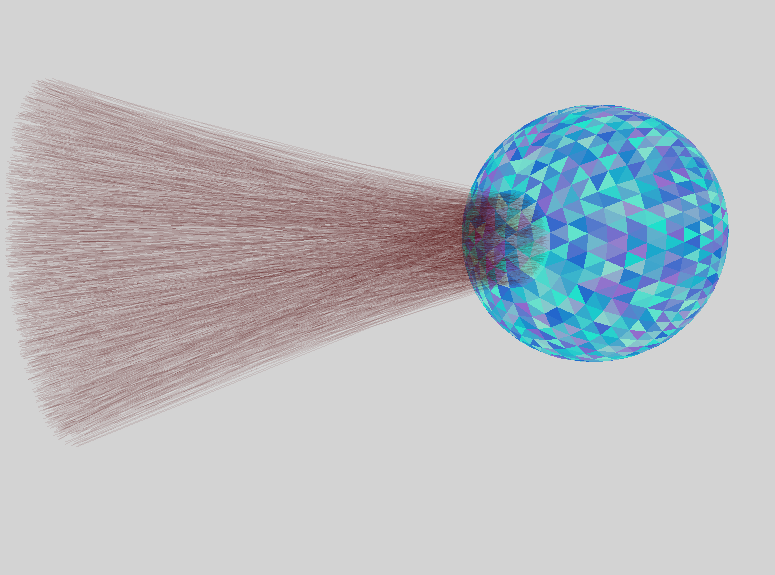
\includegraphics[scale=.2]{sphere_demo.png}
&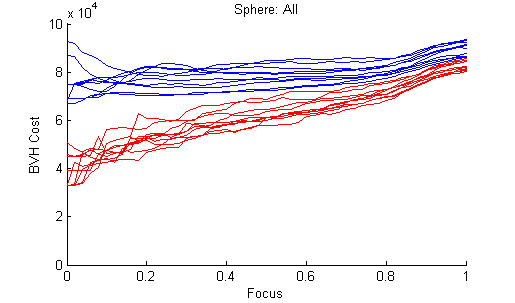
\includegraphics[scale=.35]{sphere_all.png}
&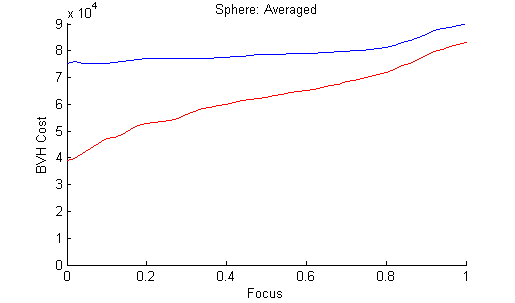
\includegraphics[scale=.35]{sphere_average.png}
\\
\hline 
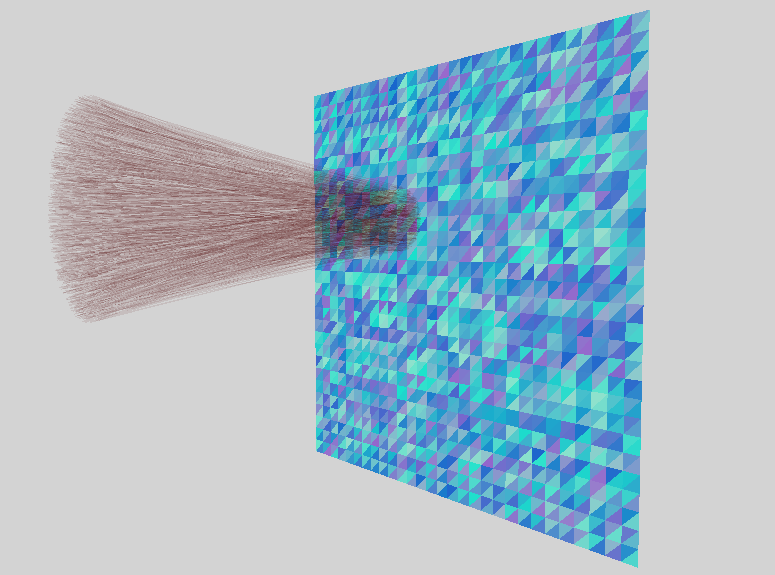
\includegraphics[scale=.2]{plane_demo.png}
&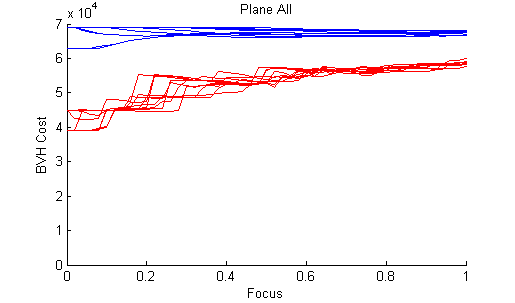
\includegraphics[scale=.35]{plane_all.png}
&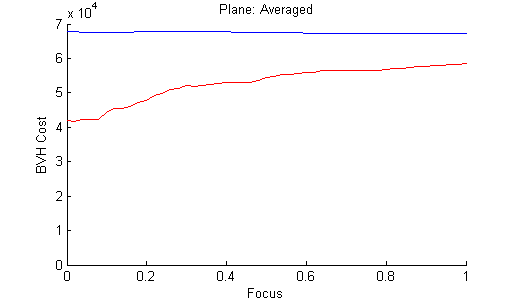
\includegraphics[scale=.35]{plane_average.png}
\\
\hline
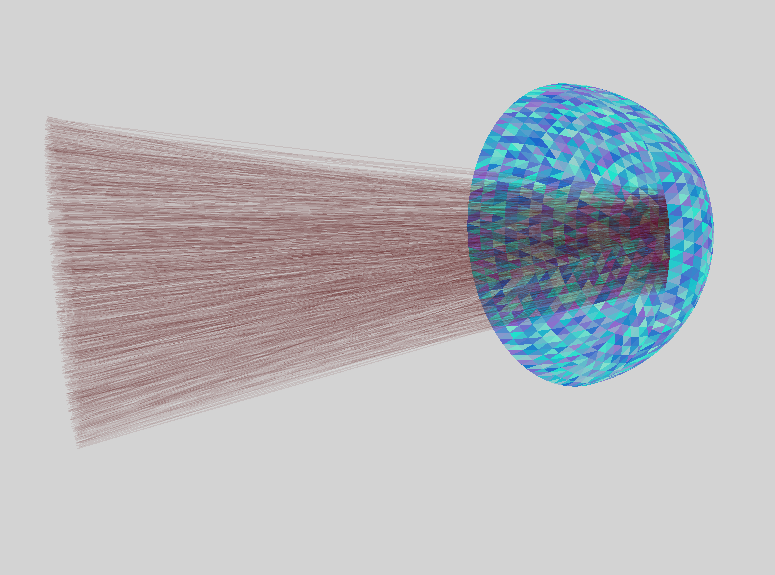
\includegraphics[scale=.2]{hemisphere_demo.png}
&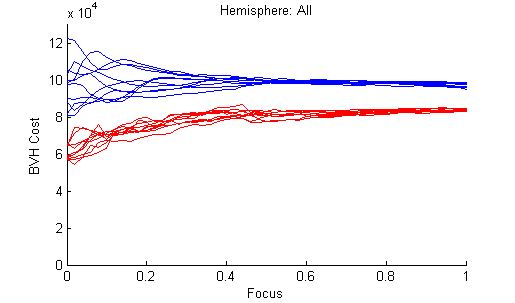
\includegraphics[scale=.35]{hemisphere_all.png}
&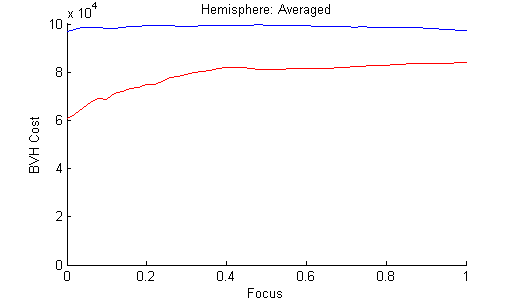
\includegraphics[scale=.35]{hemisphere_average.png}
\\
\hline
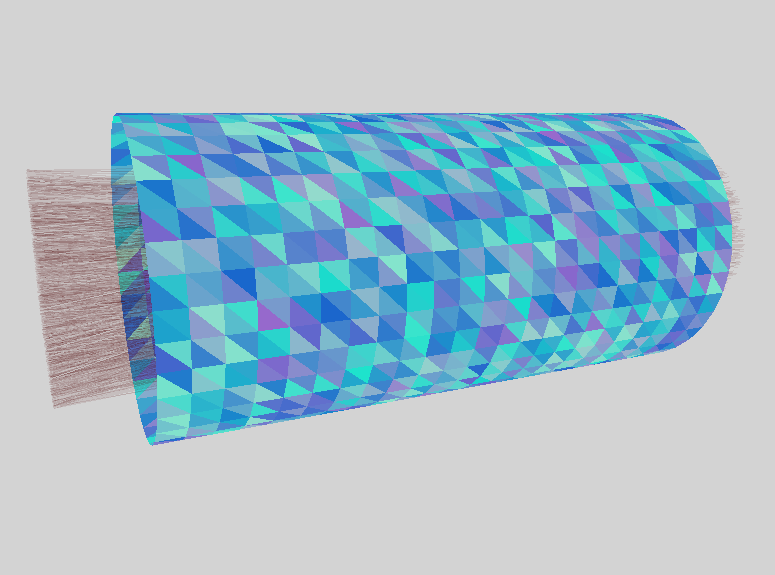
\includegraphics[scale=.2]{tube_demo.png}
&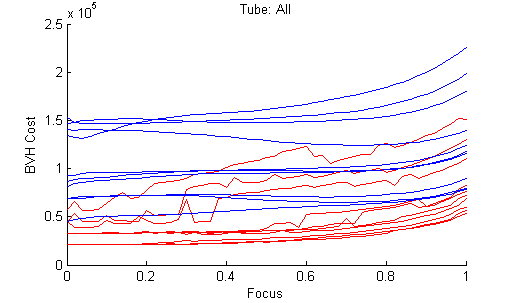
\includegraphics[scale=.35]{tube_all.png}
&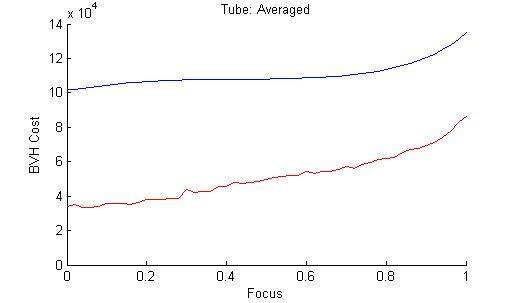
\includegraphics[scale=.35]{tube_average.png} 
\end{tabular}
\end{figure*}

\begin{figure}
\caption{Not bad}
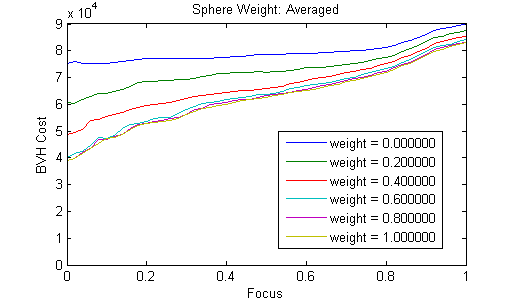
\includegraphics[scale=.6]{weight_average.png}
\end{figure}

\begin{figure*}
\caption{Not bad}
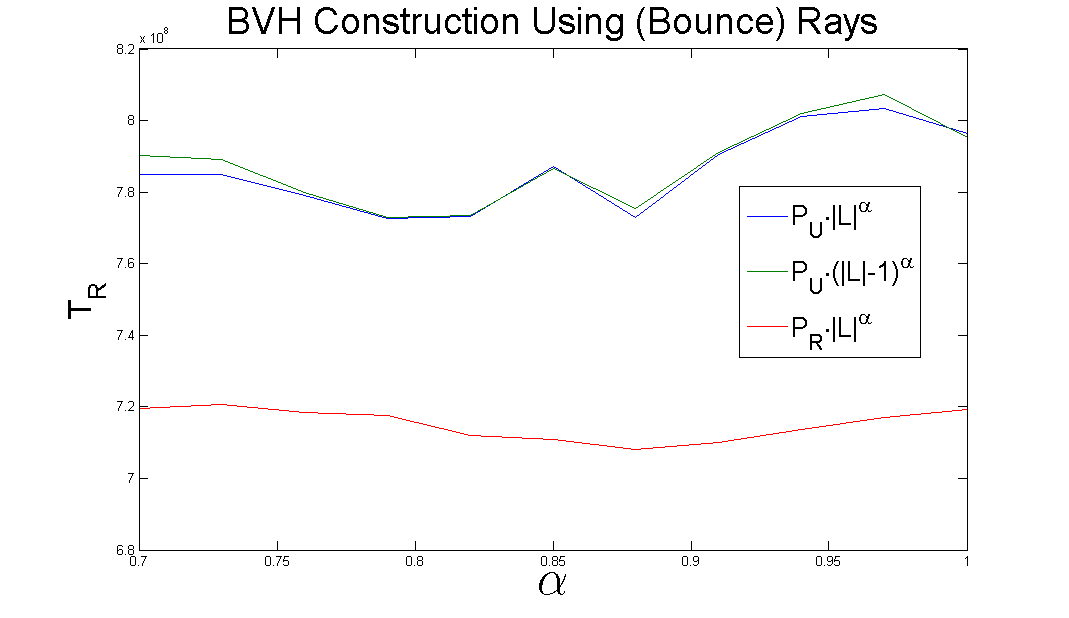
\includegraphics[scale=.6]{powerplant.png}
\end{figure*}

\section{Conclusion and Future Work}



\bibliography{final}
\bibliographystyle{plain}
\end{document}